\documentclass[10pt]{amsart}
\usepackage[a4paper,margin=20mm]{geometry}
\usepackage{amsmath,amssymb,amsthm,mathtools,mathrsfs}
\usepackage{enumitem}
\usepackage{tikz}
\usepackage{hyperref}
\newtheorem{theorem}{Theorem}[section]
\newtheorem{lemma}[theorem]{Lemma}
\newtheorem{corollary}[theorem]{Corollary}
\newtheorem{example}[theorem]{Example}
\newtheorem{remark}[theorem]{Remark}
\newtheorem{theo*}{Theorem}
\newtheorem{coro}[theorem]{Corollary}
\newtheorem{exam}[theorem]{Example}
\newtheorem{rema}[theorem]{Remark}
\providecommand{\firstname}[1]{#1}\providecommand{\lastname}[1]{#1}\providecommand{\curraddr}[1]{}\providecommand{\urladdr}[1]{}\providecommand{\DOI}[1]{}\providecommand{\datereceived}[1]{}\providecommand{\daterevised}[1]{}\providecommand{\dateaccepted}[1]{}\providecommand{\longthanks}[1]{\thanks{#1}}
\providecommand{\cf}{cf.}

\usepackage{tikz}

\providecommand{\dobbensort}[1]{}
\providecommand{\dobbensort}[1]{}

%%%%%%%%%%%%%%%%%%%%%%%%%%%%%%%%%%%%%%%%%%%%%%%%%%%%%%%%%%%%%%%%%%%%%%%%%%%%%%
%% New definitions (macros, mostly for mathematics)
%%%%%%%%%%%%%%%%%%%%%%%%%%%%%%%%%%%%%%%%%%%%%%%%%%%%%%%%%%%%%%%%%%%%%%%%%%%%%%
\newcommand{\Z}{\ensuremath{\mathbb{Z}}}
\newcommand{\R}{\ensuremath{\mathbb{R}}}
\newcommand{\transp}{\mathsf{T}}

\newcommand{\one}{\ensuremath{\mathbf{1}}}

\DeclareMathOperator{\tw}{tw}
\DeclareMathOperator{\Div}{Div}
\DeclareMathOperator{\Rat}{Rat}

\DeclareMathOperator{\Prin}{Prin}
\DeclareMathOperator{\Col}{Col}

\DeclareMathOperator{\todiv}{div}

\DeclareMathOperator{\dgon}{dgon}
\DeclareMathOperator{\sgon}{sgon}

\DeclareMathOperator{\supp}{supp}
\DeclareMathOperator{\rank}{rank}

\newcommand*{\B}{\mathcal{B}}
%\newcommand*{\order}[1]{\left|\left|#1\right|\right|}
\newcommand*{\order}[1]{\left\Vert#1\right\Vert}

%%%%%%%%%%%%%%%%%%%%%%%%%%%%%%%%%%%%%%%%%%%%%%%%%%%%%%%%%%%%%%%%%%%%%%%%%%%%%%
%% TikZ
%%%%%%%%%%%%%%%%%%%%%%%%%%%%%%%%%%%%%%%%%%%%%%%%%%%%%%%%%%%%%%%%%%%%%%%%%%%%%%
\newcommand{\hittingsetTikZ}
{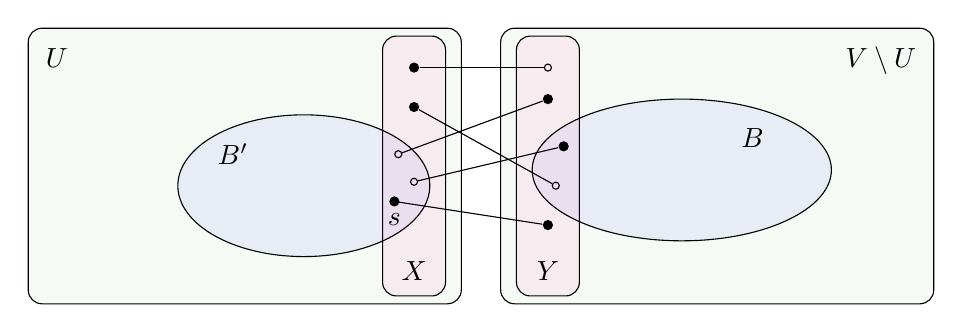
\begin{tikzpicture}[punt/.style={draw,circle,inner sep=.9pt},
	 grootpunt/.style={fill,circle,inner sep=1.3pt}]
		
		\draw[rounded corners=5pt,fill=green!30!gray!6] (0,0) rectangle (5.5,3.5);
		\node[anchor=base west] at (0.1,3) {$U$};
		
		\draw[rounded corners=5pt,fill=green!30!gray!6] (6,0) rectangle (11.5,3.5);
		\node[anchor=base east] at (11.4,3) {$V\setminus U$};
		
		\draw[rounded corners=5pt,fill=purple!60!gray!10] (4.5,0.1) rectangle (5.3,3.4);
		\node[anchor=base] at (4.9,0.3) {$X$};
		
		\draw[rounded corners=5pt,fill=purple!60!gray!10] (6.2,0.1) rectangle (7,3.4);
		\node[anchor=base] at (6.6,0.3) {$Y$};
		
		\draw[fill=blue,fill opacity=0.05] (3.5,1.5) ellipse (16mm and 9mm);
		\node at (2.6,1.9) {$B'$};
		
		\draw[fill=blue,fill opacity=0.05] (8.3,1.7) ellipse (19mm and 9mm);
		\node at (9.2,2.1) {$B$};
	
		\node[grootpunt] (A1) at (4.9,3) {};
		\node[punt] (B1) at (6.6,3) {};
		\draw (A1) -- (B1);
		\node[grootpunt] (B2) at (6.6,2.6) {};
		\node[punt] (A2) at (4.7,1.9) {};
		\draw (B2) -- (A2);
		\node[grootpunt] (B3) at (6.8,2) {};
		\node[punt] (A3) at (4.9,1.55) {};
		\draw (B3) -- (A3);
		\node[grootpunt] (A4) at (4.9,2.5) {};
		\node[punt] (B4) at (6.7,1.5) {};
		\draw (A4) -- (B4);
		\node[grootpunt,label=below:$s$,outer sep=-1pt] (s) at (4.65,1.3) {};
		\node[grootpunt] (B5) at (6.6,1.0) {};
		\draw (s) -- (B5);
\end{tikzpicture}}



\newcommand{\PetersenTikZa}
{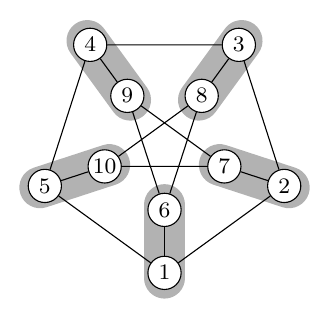
\begin{tikzpicture}[x=0.8cm,y=0.8cm]
\tikzstyle{vertex}=[circle, draw, fill=white, inner sep=0pt, minimum width=12pt, font=\footnotesize]
\tikzstyle{edge} = [] 
\tikzstyle{fedge} = [line width=15pt, color=black!30!white, shorten <=-8pt, shorten >=-8pt, line cap=round] 

 \node[vertex] (a) at (0,-1) {$6$};
 \node[vertex] (b) at (0.95,-0.31) {$7$};
 \node[vertex] (c) at (0.59,0.81) {$8$};
 \node[vertex] (d) at (-0.59,0.81) {$9$};
 \node[vertex] (e) at (-0.95,-0.31) {$10$};

 \node[vertex] (A) at (0,-2) {$1$};
 \node[vertex] (B) at (1.9,-0.62) {$2$};
 \node[vertex] (C) at (1.18,1.62) {$3$};
 \node[vertex] (D) at (-1.18,1.62) {$4$};
 \node[vertex] (E) at (-1.9,-0.62) {$5$};

 \draw[fedge] (a)--(A);
 \draw[fedge] (b)--(B);
 \draw[fedge] (c)--(C);
 \draw[fedge] (d)--(D);
 \draw[fedge] (e)--(E);

 \node[vertex] (a) at (0,-1) {$6$};
 \node[vertex] (b) at (0.95,-0.31) {$7$};
 \node[vertex] (c) at (0.59,0.81) {$8$};
 \node[vertex] (d) at (-0.59,0.81) {$9$};
 \node[vertex] (e) at (-0.95,-0.31) {$10$};

 \node[vertex] (A) at (0,-2) {$1$};
 \node[vertex] (B) at (1.9,-0.62) {$2$};
 \node[vertex] (C) at (1.18,1.62) {$3$};
 \node[vertex] (D) at (-1.18,1.62) {$4$};
 \node[vertex] (E) at (-1.9,-0.62) {$5$};

 
 \draw[edge] (a)--(A);
 \draw[edge] (b)--(B);
 \draw[edge] (c)--(C);
 \draw[edge] (d)--(D);
 \draw[edge] (e)--(E);
 
 
 \draw[edge] (a)--(c)--(e)--(b)--(d)--(a);
 \draw[edge] (A)--(B)--(C)--(D)--(E)--(A);
\end{tikzpicture}}





\newcommand{\PetersenTikZb}{
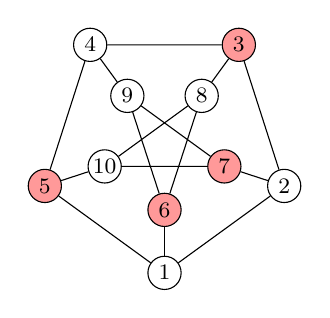
\begin{tikzpicture}[x=0.8cm,y=0.8cm]
\tikzstyle{vertex}=[circle, draw, fill=white, inner sep=0pt, minimum width=12pt, font=\footnotesize]
\tikzstyle{rvertex}=[circle, draw, fill=white!60!red, inner sep=0pt, minimum width=12pt, font=\footnotesize]

\tikzstyle{edge} = [] 
\tikzstyle{fedge} = [line width=15pt, color=black!30!white, shorten <=-8pt, shorten >=-8pt, line cap=round] 

 \node[rvertex] (a) at (0,-1) {$6$};
 \node[rvertex] (b) at (0.95,-0.31) {$7$};
 \node[vertex] (c) at (0.59,0.81) {$8$};
 \node[vertex] (d) at (-0.59,0.81) {$9$};
 \node[vertex] (e) at (-0.95,-0.31) {$10$};

 \node[vertex] (A) at (0,-2) {$1$};
 \node[vertex] (B) at (1.9,-0.62) {$2$};
 \node[rvertex] (C) at (1.18,1.62) {$3$};
 \node[vertex] (D) at (-1.18,1.62) {$4$};
 \node[rvertex] (E) at (-1.9,-0.62) {$5$};

 \draw[edge] (a)--(A);
 \draw[edge] (b)--(B);
 \draw[edge] (c)--(C);
 \draw[edge] (d)--(D);
 \draw[edge] (e)--(E);
 
 
 \draw[edge] (a)--(c)--(e)--(b)--(d)--(a);
 \draw[edge] (A)--(B)--(C)--(D)--(E)--(A);
\end{tikzpicture}}
%%%%%%%%%%%%%%%%%%%%%%%%%%%%%%%%%%



%%%%%%%%% a placer avant \usepackage[no-math]{fontspec}\setmainfont{Latin Modern Roman}[SmallCapsFont=lmromancaps10-regular.otf]
\begin{document}\title{Treewidth is a lower bound on graph gonality}\author{Josse van Dobben de Bruyn}\author{Dion Gijswijt}\date{}\maketitle\setcounter{section}{1}
\section{Preliminaries} 
The graphs in this paper will be finite and undirected (unless stated otherwise). We allow our graphs to have multiple (parallel) edges, but no loops. We will almost exclusively consider \emph{connected} graphs. For a graph~$G$, we denote by $V(G)$ and $E(G)$ the set of vertices and edges of~$G$, respectively. By an edge~$uv$, we mean an edge with ends $u$~and~$v$. For (not necessarily disjoint) subsets~$U,W\subseteq V(G)$, we denote by $E(U,W)$ the set of edges with an end in~$U$ and an end in~$W$. For vertices~$u$ and~$v$, we use the abbreviations $E(u,v)\coloneqq E(\{u\},\{v\})$ and $E(u)\coloneqq E(\{u\},V\setminus \{u\})$. The degree of a vertex~$v$ equals the number of edges with $v$ as an endpoint and is denoted by $d_G(v)\coloneqq |E(v)|$. For a subset~$U\subseteq V(G)$, we denote by $G[U]\coloneqq (U,E(U,U))$ the subgraph of~$G$ \emph{induced by~$U$}. That is, $G[U]$ is the graph with vertex set~$U$ and edge set consisting of the edges of~$G$ with both ends in~$U$.

Let $G=(V,E)$ be a \emph{connected} graph. We can make $G$ into an \emph{oriented graph} by, for every edge~$e$, assigning one end to be the \emph{head} of~$e$ and the other end to be the \emph{tail} of~$e$. We view the edge~$e$ as oriented from its tail to its head. For a cycle~$C$ in~$G$, we then denote by $\chi_C\in \R^{E}$ the signed incidence vector defined by
\begin{equation}
\chi_C(e)=\begin{cases}
1& \text{if $e$ is traversed in forward direction by $C$,}\\
-1&\text{if $e$ is traversed in backward direction by $C$,}\\
0&\text{otherwise.}
\end{cases}
\end{equation} 
Similarly, we write $\chi_P$ for the signed incidence vector of a path~$P$.

The \emph{incidence matrix}~$M=M(G)\in \R^{V\times E}$ of~$G$ is defined by, for every~$v\in V$ and~$e\in E$, setting 
\begin{equation}
M_{v,e}\coloneqq 
\begin{cases}
1&\text{if $v$ is the head of $e$,}\\
-1&\text{if $v$ is the tail of $e$,}\\
0&\text{otherwise.}
\end{cases}
\end{equation}
\noindent The matrix~$Q=Q(G)\coloneqq MM^\transp$ is the \emph{Laplacian} of~$G$ and it is independent of the chosen orientation. Indeed, for any two vertices~$u$ and~$v$, $Q_{vv}$ equals the degree of vertex~$v$ and $Q_{uv}$ equals~$-|E(u,v)|$. The \emph{cut lattice} of~$G$ is the set~$\Z^{E}\cap \Col(M^\transp)$ of integral vectors in the column space of the transpose of~$M$. 

The following two lemmas are well-known, and can be found in many books on algebraic graph theory (for example~\cite{GodsilRoyle2001}). For the benefit of the reader, we will give the short proofs.
 
\begin{lemma}\label{clattice}
Let $f\in \Z^{E}$. Then the following are equivalent:
\begin{enumerate}[label=(\roman*)]
\item\label{lemma2.1_i} $f$ is in the cut lattice of $G$,
\item\label{lemma2.1_ii} $f^\transp\chi_C=0$ for every cycle $C$ in $G$,
\item\label{lemma2.1_iii} $f=M^\transp x$ for some $x\in \Z^{V}$.
\end{enumerate}
\end{lemma} 
\begin{proof}
The implication from~\ref{lemma2.1_iii} to~\ref{lemma2.1_i} is trivial. The implication from~\ref{lemma2.1_i} to~\ref{lemma2.1_ii} follows since $M\chi_C=0$ for every cycle~$C$. For the implication from~\ref{lemma2.1_ii} to~\ref{lemma2.1_iii}, let $f\in \Z^{E}$ satisfy the condition in~\ref{lemma2.1_ii}. Let $T$ be a spanning tree in~$G$ with root~$r$, and define $x\in \Z^V$ by $x(v)\coloneqq f^\transp\chi_{P_v}$, where $P_v$ is the path in~$T$ from~$r$ to~$v$. Now for every edge~$e=uv$ oriented from~$u$ to~$v$, we have $x(v)-x(u)=f(e)$. Hence, $f=M^\transp x$.
\end{proof}

\begin{lemma}\label{Laplacian}
The null space of~$Q$ is spanned by the all-one vector~$\one$.
\end{lemma}
\begin{proof}
Since the row sums of~$Q$ equal zero, it is clear that~$Q\one=0$. Conversely, let $x$ be in the null space of~$Q$ and suppose, for contradiction, that $x$ is not a multiple of~$\one$. Since $G$ is connected, we may choose $v\in V$ for which $x(v)$ is maximal and such that $v$ has a neighbour~$u$ with $x(u) < x(v)$. From~$Qx=0$ it follows that $d_G(v)x(v)=\sum_{w\in V\setminus\{v\}} |E(v,w)|\cdot x(w)$. On the other hand,
\begin{equation*}
\sum_{w\in V\setminus\{v\}}|E(v,w)|\cdot x(w)\ < \sum_{w\in V\setminus\{v\}}|E(v,w)|\cdot x(v)= d_G(v)x(v)
\end{equation*}
by our choice of~$v$. This is a contradiction. 
\end{proof}

 
\subsection{Divisors on graphs}
We will largely adopt notation from~\cite{BakerNorine2007}. Let $G=(V,E)$ be a connected graph. A vector~$D\in \Z^V$ is called a \emph{divisor} on~$G$. The set~$\Div(G)\coloneqq \Z^V$ denotes the set of all divisors on~$G$. For a divisor~$D\in \Div(G)$ we call $\deg(D)\coloneqq \sum_{v\in V}D(v)$ the \emph{degree} of~$D$. A divisor~$D$ is said to be \emph{effective} if it is nonnegative, that is, $D(v)\geq 0$ for all~$v\in V$. We denote by $\Div_+(G)$ the set of effective divisors on~$G$ and by $\Div_+^k(G)$ the set of effective divisors of degree~$k$. We denote by $\supp(D)\coloneqq \{v\in V\mid D(v)\neq 0\}$ the \emph{support} of~$D$.

We call two divisors~$D$ and~$D'$ \emph{equivalent} and write $D\sim D'$ if there is an integer vector~$x\in \Z^V$ such that $D-D'=Q(G)x$. Clearly, this is indeed an equivalence relation. Observe that equivalent divisors have equal degree as $Q(G)$ has column sums equal to zero. 

We will often consider the situation where $x$ is the incidence vector of a subset~$U$ of~$V$, that is, $D'=D-Q(G)\one_U$. Observe that in this case 
\begin{equation}
D'(v)=\begin{cases}D(v)-|E(\{v\},V\setminus U)|&\text{if $v\in U$},\\D(v)+|E(\{v\},U)|&\text{if $v\in V\setminus U$.}\end{cases}
\end{equation}
In particular, $D'(v)\leq D(v)$ if $v\in U$ and $D'(v)\geq D(v)$ if $v\in V\setminus U$. In terms of chip firing, we move one chip along each edge in the cut~$E(U,V\setminus U)$. The following lemma shows that for equivalent effective divisors~$D$ and~$D'$, we can obtain $D'$ from~$D$ by a sequence of steps of this form such that each intermediate divisor is effective as well.

\begin{lemma}\label{chain}
Let $D_0$ and~$D$ be equivalent effective divisors satisfying~$D \neq D_0$. There is a chain of sets~$\emptyset\subsetneq U_1\subseteq U_2\subseteq \cdots\subseteq U_k\subsetneq V$ such that $D_t\coloneqq D-Q(G)(\sum_{i=1}^t \one_{U_i})$ is effective for every~$t=1,\ldots,k$ and such that~$D_k=D$. Moreover, this chain is unique.
\end{lemma}
\begin{proof}
Since~$D_0\sim D$, there exists an~$x\in \Z^V$ such that~$D_0-Q(G)x=D$. By Lemma~\ref{Laplacian}, $x$ is unique up to integral multiples of~$\one$. Hence, there is a unique such $x$ with the additional property that $x\geq 0$ and $\supp(x)\neq V$. Let $k\coloneqq \max\{x(v)\mid v\in V\}$ and define $U_i\coloneqq \{v\in V\mid x(v)\geq k-i+1\}$ for $i=1,\ldots, k$. We have $\emptyset\subsetneq U_1\subseteq U_2\subseteq \cdots\subseteq U_k\subsetneq V$ as required. Also, $\sum_{i=1}^k \one_{U_i}=x$ and hence $D_k=D_0-Q(G)x=D$.

Consider any~$t\in \{1,\ldots, k-1\}$. To show effectiveness of~$D_t$, consider any~$v\in V$. If $v\not\in U_t$, then $D_0(v)\leq D_1(v)\leq \cdots\leq D_t(v)$, hence~$D_t(v)\geq 0$. If~$v\in U_t$, then $D_t(v)\geq D_{t+1}(v)\geq \cdots \geq D_k(v)$, hence~$D_t(v)\geq 0$. 

Uniqueness follows directly from the uniqueness of an~$x\in \Z^V$ for which $x\geq 0$, $\supp(x)\neq V$ and $D_0-Q(G)x=D$, in combination with the uniqueness of the decomposition~$x=\sum_{i=1}^k\one_{U_i}$ as a sum of characteristic vectors of a chain~$\emptyset\subsetneq U_1\subseteq U_2\subseteq \cdots\subseteq U_k\subsetneq V$.
\end{proof}

The \emph{rank} of a divisor~$D$ is defined as
\begin{multline}
\rank(D)\coloneqq \max\{k\mid \text{$D-D'$ is equivalent to an effective divisor}\\\text{ for every~$D'\in\Div_+^k$}\}.
\end{multline}
Observe that equivalent divisors have equal rank and that $\rank(D)\leq \deg(D)$.

Following Baker~\cite{Baker2008}, we define the \emph{gonality} of~$G$ by
\begin{equation}
\dgon(G)\coloneqq \min\{k\mid \text{there is a divisor of degree~$k$ on~$G$ with positive rank}\}.
\end{equation} 


An effective divisor~$D$ is called \emph{$v$-reduced} if for any nonempty subset~$U\subseteq V\setminus \{v\}$ the divisor~$D-Q(G)\one_U$ is not effective\footnote{The definition of $v$-reduced divisor can be extended to all divisors by allowing $D(v)$ to be negative for a $v$-reduced divisor~$D$ as is done in~\cite{BakerNorine2007}. However, in this paper we will mostly deal with effective divisors.}. In other words, for every nonempty~$U\subseteq V\setminus \{v\}$ there is a~$u\in U$ with $D(u)<|E(\{u\}, V\setminus U)|$. 

\begin{lemma}[{\cite[Proposition~3.1]{BakerNorine2007}}]\label{reduction}
Let $v\in V$ and let $D$ be an effective divisor on~$G$. Then there is a unique $v$-reduced divisor equivalent to~$D$.
\end{lemma}

\begin{proof}
For any divisor~$D' \sim D$, there is a unique $x_{D'}\in \{x\in \Z^V\mid x(v)=0\}$ such that~$D'=D-Q(G)x_{D'}$ by Lemma~\ref{Laplacian}. Let 
\begin{equation}
S\coloneqq \{x_{D'}\mid D'\text{ is effective and equivalent to~$D$}\}.
\end{equation}
The set~$S$ is finite since the number of effective divisors equivalent to~$D$ is finite. The set~$S$ is nonempty as it contains the zero vector. Choose~$x_{D'}\in S$ maximizing $\sum_{u\in V} x_{D'}(u)$. Then $D'$ is $v$-reduced because for any nonempty~$U\subseteq V\setminus \{v\}$, the vector~$x_{D'}+\one_U$ is not in~$S$ by the choice of~$x_{D'}$. 

To show uniqueness, let $D$ and~$D'$ be two different, but equivalent effective divisors. It suffices to show that $D$ and~$D'$ are not both $v$-reduced. By Lemma~\ref{chain} there are sets~$\emptyset\subsetneq U_1\subseteq\cdots\subseteq U_k\subsetneq V$ such that $D-Q(G)\one_{U_1}$ and $D'+Q(G)\one_{U_k}=D'-Q(G)\one_{V\setminus U_k}$ are effective. If $v\not\in U_1$, then $D$ is not $v$-reduced. If $v\in U_1$, then $v\not\in V\setminus U_k\subseteq V\setminus U_1$ and hence $D'$ is not $v$-reduced.
\end{proof}
\begin{rema}
Observe that if $D$ is a $v$-reduced divisor, then $D(v)\geq D'(v)$ for any effective divisor~$D'\sim D$. Indeed, by Lemma~\ref{chain} we obtain $D'$ from~$D$ by firing on a chain of sets $U_1\subseteq\cdots\subseteq U_t$ and, since $D$ is $v$-reduced, we have $v\in U_1$. We conclude that if $D$ is a $v$ reduced divisor of positive rank, we have $D(v)\geq 1$. 
\end{rema}

We say that an effective divisor~$D$ \emph{covers} $v\in V$ if there is an effective divisor~$D'$ equivalent to~$D$ with $v\in \supp(D')$. We call a nonempty subset~$S\subseteq V$ a \emph{strong separator} if for each component~$C$ of $G[V\setminus S]$ we have that $C$ is a tree and $|E(\{s\},V(C))|\leq 1$ for every~$s\in S$. The following lemma is similar to a theorem of Luo~\cite{Luo2011} on rank determining sets in the context of metric graphs.

\begin{lemma}\label{Luotype}
Let $S$ be a strong separator of~$G$ and let $D$ be an effective divisor covering every~$s\in S$. Then $D$ has positive rank. 
\end{lemma}
\begin{proof}
Since any superset of a strong separator is again a strong separator, we may assume that
\begin{equation}
	S=\{s\in V\mid \text{$s$ is covered by $D$}\}. \label{eqn:S-assumption}
\end{equation}
We have to show that $S=V$. 

Suppose not. Let $C$ be a component of $G[V\setminus S]$ and let $S'\coloneqq \{s\in S: |E(\{s\},V(C))|=1\}$. Since $G$ is connected, $S'$ is not empty, so we may take $s\in S'$ and assume that $D$ is $s$-reduced. If $S'\subseteq \supp(D)$, then $D+Q(G)\one_{V(C)}$ is effective and has support on at least one vertex in $V(C)\subseteq V\setminus S$, but this contradicts~\eqref{eqn:S-assumption}. Therefore, $S' \not\subseteq \supp(D)$. 

Choose $t\in S'\setminus \supp(D)$. By~\eqref{eqn:S-assumption}, $t$ is covered by~$D$. However, $t$ is not in the support of~$D$, so in particular $D$ is not $t$-reduced. Let $a$ and $b$ be the unique neighbours of $s$~and~$t$ in~$V(C)$, respectively, and let $P=(s,a,\ldots,b,t)$ be the path from~$s$ to~$t$ with its interior points in~$V(C)$. Since $D$ is $s$-reduced, but not $t$-reduced, there is a set~$U\subseteq V$ with $s\in U$, $t\not\in U$ such that $D'\coloneqq D-Q(G)\one_U$ is effective. The cut~$E(U,V\setminus U)$ must intersect some edge~$e=uv$ of the path~$P$, and we find that $D(u)\geq 1$ and $D'(v)\geq 1$. This contradicts~\eqref{eqn:S-assumption}, since at least one of $u$~and~$v$ is in~$V(C)\subseteq V\setminus S$.
\end{proof}

\begin{coro}
\label{rankdetermining}
If $H$ is a subdivision of~$G$ and $D$ is a divisor on~$H$ that covers all~$v\in V(G)$, then $D$ has positive rank.
\end{coro}

Corollary~\ref{rankdetermining} can be seen as a discrete analogue of~\cite[Theorem~1.6]{Luo2011}\footnote{In the preprint of~\cite{Luo2011} (\cf \href{https://arxiv.org/abs/0906.2807v2}{arXiv:0906.2807v2}), this is Theorem~1.5 (instead of~1.6).}.

\subsection{Treewidth}
The notion of \emph{treewidth} was first introduced by Halin~\cite{Halin1976} and later rediscovered by Robertson and Seymour~\cite{RobertsonSeymour1990} as part of their graph minor theory. There are several equivalent definitions of treewidth. We will follow Diestel~\cite{DiestelGraphTheory}, and define treewidth in terms of tree-decompositions.

Let $G=(V,E)$ be a graph (we allow multiple edges and loops). Let $(X_i)_{i\in I}$ be a family of vertex sets $X_i\subseteq V$ indexed by the nodes of a tree $T=(I,F)$. The pair $(T,(X_i)_{i\in I})$ is a \emph{tree decomposition} of $G$ if it satisfies the following conditions: 
\begin{enumerate}[label=(\roman*)]
 \item $\bigcup_{i\in I} X_i = V$;
 \item for every edge $e=vw\in E$ there is an $i\in I$ with $v,w\in X_i$;
 \item if $i,j,k\in I$ and node $j$ is on the path in $T$ between nodes $i$ and $k$, then $X_i\cap X_k\subseteq X_j$.
\end{enumerate}
The \emph{width} of the tree decomposition is $\max_{i\in I} |X_i|-1$. The \emph{treewidth} of a $G$ is the minimum width of a tree decomposition of $G$. 


In order to use treewidth as a lower bound, we will use a characterisation of treewidth by Seymour and Thomas~\cite{SeymourThomas1993} in terms of ``brambles''.\footnote{The article of Seymour and Thomas~\cite{SeymourThomas1993} used the term \emph{screen} instead of \emph{bramble}, but the latter has since become the standard.} Let $G=(V,E)$ be a graph, and let $2^V$ denote the power set of $V$. A set $\B\subseteq 2^V\setminus\{\emptyset\}$ is called a \emph{bramble} if for any $B,B'\in \B$ the induced subgraph $G[B\cup B']$ is connected. In particular, $G[B]$ is connected for every $B\in \B$. For any $B,B'\in \B$, either $B\cap B'\neq \emptyset$, or $B\cap B'=\emptyset$ and there is an edge in $E(B,B')$. In the latter case, we say that $B$ and $B'$ \emph{touch}.
A set $S\subseteq V$ is called a \emph{hitting set} for $\B$ if it has nonempty intersection with every member of $\B$. The \emph{order} of $\B$, denoted $\order{\B}$, is the minimum size of a hitting set for $\B$. That is:
\begin{equation}
\order{\B}\coloneqq \min \{|S| : S\subseteq V, S\cap B\neq\emptyset \text{ for all $B\in \B$}\}.
\end{equation}

The following theorem by Seymour and Thomas~\cite{SeymourThomas1993} gives a min-max characterisation of treewidth.

\begin{theorem}[{treewidth duality, \cite[Theorem~1.4]{SeymourThomas1993}}]
Let $k\geq 0$ be an integer. A graph $G$ has treewidth at least $k$ if and only if it has a bramble of order at least $k + 1$.
\end{theorem} 

\begin{rema}
We note that the treewidth of a graph is equal to the treewidth of the underlying simple graph, as can be seen directly from the definition. It is well-known that treewidth is monotone under taking minors (see for example~\cite{DiestelGraphTheory}). That is, removing or contracting edges can only decrease treewidth. In particular, if $H$ is a subdivision of $G$, then $\tw(G)\leq \tw(H)$. 


\end{rema}
We refer the interested reader to Chapter~12 in~\cite{DiestelGraphTheory} for an excellent exposition of treewidth and its role in the graph minor theory.

\section{Proof of the main theorem}
In this section we prove our main theorem.
\begin{theorem}\label{main}
Let $G=(V,E)$ be a connected graph. Then $\dgon(G)\geq \tw(G)$.
\end{theorem} 

We start by stating and proving two lemmas.
\begin{lemma}\label{oneside}
Let $D,D'$ be effective divisors such that $D'=D-Q(G)\one_U$ for some subset $U\subseteq V$. Let $B\subseteq V$ be such that $G[B]$ is connected. Suppose that $B\cap \supp(D)$ is nonempty, but $B\cap \supp(D')$ is empty. Then $B\subseteq U$.
\end{lemma}
\begin{proof}
Clearly, $B$ cannot be a subset of $V\setminus U$, because otherwise $D'(v)\geq D(v)$ for every $v\in B$. Now suppose that $B\cap U$ and $B\setminus U$ are both nonempty. Since $G[B]$ is connected, there is an edge $uv$ with $u\in B\cap U$ and $v\in B\setminus U$. But then $D'(v)=(D-Q(G)\one_U)(v)\geq D(v)+1\geq 1$ since $u\in U$ is a neighbour of $v\in V\setminus U$. This is a contradiction as well, so we see that $B\subseteq U$ must hold.
\end{proof}

\begin{lemma}\label{brambleseparation}
Let $\B$ be a bramble in $G$ and let $U\subseteq V$. Suppose that there exist $B,B'\in \B$ such that $B\subseteq V\setminus U$ and $B'\subseteq U$. Then $|E(U,V\setminus U)|+1\geq \order{\B}$.
\end{lemma}

\begin{proof}
We will construct a hitting set for $\B$ of size at most $|E(U,V\setminus U)|+1$.
Let $F\coloneqq E(U,V\setminus U)$ be the cut determined by $U$ and let $H\coloneqq (V,F)$. Let 
\[ 
X\coloneqq \{v\in U\mid d_H(v)\geq 1\}\qquad\text{and}\qquad Y\coloneqq \{v\in V\setminus U\mid d_H(v)\geq 1\}
\]
be the ``shores'' of the cut $F$. Let $B\in \B$ be such that $B\subseteq V\setminus U$. Let $\B'\coloneqq \{B'\in \B\mid B'\subseteq U\}$. By assumption, $\B'$ is nonempty. Choose $B'\in \B'$ for which $B'\cap X$ is inclusion-wise minimal. Observe that $B'\cap X$ is nonempty, since $B'$ must touch $B$. 

We now define a hitting set~$S$ for~$\B$ as follows. Add an arbitrary element~$s$ from \hbox{$B'\cap X$} to~$S$. For each edge~$xy\in E(X,Y)$ with $x\in X, y\in Y$, we add $x$ to~$S$ if $x\not\in B'$, and otherwise we add $y$ to~$S$. Hence $|S|\leq 1+|F|$. See Figure~\ref{hittingset} for a depiction of the situation.

\begin{figure}[htb]\centering
\hittingsetTikZ
\caption{The hitting set $S$ for the bramble $\B$ is formed by the black vertices.\label{hittingset}}
\end{figure}
%\medskip

To prove that $S$ covers $\B$, consider any $A\in \B$. First observe that $A$ intersects $X\cup Y$. Otherwise, we would have $A\subseteq U\setminus X$ or $A\subseteq (V\setminus U)\setminus Y$ as $G[A]$ is connected. In the first case $G[A\cup B]$ is not connected and in the second case $G[A\cup B']$ is not connected. In both cases, this contradicts the fact that $\B$ is a bramble.

We consider the following three cases. 
\begin{itemize}
\item Case $A\cap Y=\emptyset$.\quad In this case $A\subseteq U$. By the choice of $B'$, we have either $B'\cap X\subseteq A\cap X$ and hence $s\in A$, or there exists an $x\in (X\cap A)\setminus B'$, which implies that $x\in S$. In both situations $S$ intersects $A$.
\item Case $A\cap X=\emptyset$.\quad In this case $A\subseteq (V\setminus U)$. Since $A$ touches $B'$, there must be an edge $e=xy$ with $x\in B'\cap X$ and $y\in A\cap Y$. By construction of $S$ we have $y\in S$. Hence, $S$ intersects $A$.
\item Case $A\cap X\neq \emptyset$ and $A\cap Y\neq \emptyset$.\quad Since $G[A]$ is connected, there is an edge $e=xy$ with $x\in X$, $y\in Y$ and $x,y\in A$. Since $S$ contains at least one endpoint from each edge in $F$, the set $S$ must intersect $A$.
\end{itemize}
We conclude that $S$ is a hitting set for $\B$ of size at most $|E(U,V\setminus U)|+1$, which proves the lemma.
\end{proof}

\noindent We now prove the main theorem.
\begin{proof}[Proof of Theorem~\ref{main}]
Let $\B$ be a bramble in $G$ of maximum order. That is, $\order{\B} = \tw(G)+1$. Let $D'$ be an effective divisor of positive rank and degree $\dgon(G)$. Among the effective divisors equivalent to $D'$, we choose $D$ such that $\supp(D)$ intersects a maximum number of sets in $\B$. If $\supp(D)$ is a hitting set for $\B$, then we are done:
\begin{equation}
\dgon(G)=\deg(D) \geq |\supp(D)| \geq \order{\B} = \tw(G)+1.
\end{equation}

We may therefore suppose that $B\in\B$ is not intersected by $\supp(D)$ and let $v\in B$. Since $D$ has positive rank and $D(v)=0$, it follows that $D$ is not $v$-reduced. Hence, by Lemma~\ref{chain}, there exist a chain $\emptyset\subsetneq U_1\subseteq\ldots\subseteq U_k\subseteq V\setminus{\{v\}}$ and a sequence of equivalent effective divisors $D_0\coloneqq D,D_1,\ldots,D_k$ such that $D_k$ is $v$-reduced and for every $i=1,\ldots, k$ we have $D_i=D_{i-1}-Q(G)\one_{U_i}$. Since $D$ has positive rank, $\supp(D_k)$ contains $v$ and hence intersects $B$.

Let $i\leq k$ be the smallest index such that there is a $B'\in \B$ that is intersected by $\supp(D_0)$ but not by $\supp(D_i)$. Such an index exists, since otherwise $\supp(D_k)$ intersects more members of $\B$ then $\supp(D_0)$, contradicting our choice of $D=D_0$. From $B'\cap \supp(D_{i-1})\neq \emptyset$ and $B'\cap \supp(D_{i})=\emptyset$ it follows by Lemma~\ref{oneside} that $B'\subseteq U_i$. 

%\looseness-1
By definition of $i$, the set $\supp(D_{i-1})$ intersects every member of $\B$ that is intersected by $\supp(D)$. By our choice of $D$, the set $\supp(D)$ intersects at least as many members of $\B$ as $\supp(D_{i-1})$ does. Hence it follows that $\supp(D_{i-1})$ does not intersect~$B$. 

Since $\supp(D_k)$ does intersect $B$, there is an index $j\geq i$ such that $B\cap \supp(D_{j-1})=\emptyset$ and $B\cap \supp(D_{j})\neq\emptyset$. Hence, since $D_{j-1}=D_j-Q(G)\one_{V\setminus U_j}$, we have $B\subseteq V\setminus U_j$ by Lemma~\ref{oneside}. This implies that also $B\subseteq V\setminus U_i$. 

Since $B\subseteq V\setminus U_i$ and $B'\subseteq U_i$, it follows by Lemma~\ref{brambleseparation} that $|E(U_i,V\setminus U_i)|\geq \order{\B}-1$. Since 
\begin{equation}
\deg (D_{i-1})\geq \sum_{u\in U_i}D_{i-1}(u)\geq |E(U_i,V\setminus U_i)|,
\end{equation}
it follows that $\dgon(G)=\deg(D) = \deg(D_{i-1}) \geq \order{\B} - 1 = \tw(G)$.
\end{proof}

\begin{thebibliography}{99}
\bibitem[1]{Baker2008} Matthew Baker, Specialization of linear systems from curves to graphs, Algebra Number Theory 2 (2008), no. 6, 613–653, With an appendix by Brian Conrad. \url{https://doi.org/10.2140/ant.2008.2.613}
\bibitem[2]{BakerNorine2007} Matthew Baker and Serguei Norine, Riemann–Roch and Abel–Jacobi theory on a finite graph, Adv. Math. 215 (2007), no. 2, 766–788. \url{https://doi.org/10.1016/j.aim.2007.04.012}
\bibitem[3]{BakerNorine2009} , Harmonic morphisms and hyperelliptic graphs, Int. Math. Res. Not. IMRN (2009), no. 15, 2914–2955. \url{https://doi.org/10.1093/imrn/rnp037}
\bibitem[4]{Biggs} Norman L. Biggs, Chip-firing and the critical group of a graph, J. Algebraic Combin. 9 (1999), no. 1, 25–45. \url{https://doi.org/10.1023/A:1018611014097}
\bibitem[5]{BLS1991} Anders Björner, László Lovász, and Peter W. Shor, Chip-firing games on graphs, European J. Combin. 12 (1991), no. 4, 283–291. \url{https://doi.org/10.1016/S0195-6698(13)80111-4}
\bibitem[6]{Caporaso2012} Lucia Caporaso, Gonality of algebraic curves and graphs, in Algebraic and complex geometry, Springer Proc. Math. Stat., vol. 71, Springer, Cham, 2014, pp. 77–108. \url{https://doi.org/10.1007/978-3-319-05404-9_4}
\bibitem[7]{Chan} Melody Chan, Tropical hyperelliptic curves, J. Algebraic Combin. 37 (2013), no. 2, 331–359. \url{https://doi.org/10.1007/s10801-012-0369-x}
\bibitem[8]{SunilKavitha2006} L. Sunil Chandran and Telikepalli Kavitha, The treewidth and pathwidth of hypercubes, Discrete Math. 306 (2006), no. 3, 359–365. \url{https://doi.org/10.1016/j.disc.2005.12.011}
\bibitem[9]{CornelissenKatoKool2012} Gunther Cornelissen, Fumiharu Kato, and Janne Kool, A combinatorial Li–Yau inequality and rational points on curves, Math. Ann. 361 (2015), no. 1-2, 211–258. \url{https://doi.org/10.1007/s00208-014-1067-x}
\bibitem[10]{DiestelGraphTheory} Reinhard Diestel, Graph theory, fourth ed., Graduate Texts in Mathematics, vol. 173, Springer, Heidelberg, 2012. \url{https://doi.org/10.1007/978-3-642-14279-6}
\bibitem[11]{vanDobbendeBruyn2012} Josse van Dobben de Bruyn, Reduced divisors and gonality in finite graphs, Bachelor thesis, Leiden University, 2012, https://www.math.leidenuniv.nl/scripties/BachvanDobbendeBruyn. pdf. 
\bibitem[12]{gathmannkerber} Andreas Gathmann and Michael Kerber, A Riemann–Roch theorem in tropical geometry, Math. Z. 259 (2008), no. 1, 217–230. \url{https://doi.org/10.1007/s00209-007-0222-4}
\bibitem[13]{GodsilRoyle2001} Chris Godsil and Gordon Royle, Algebraic graph theory, Graduate Texts in Mathematics, vol. 207, Springer-Verlag, New York, 2001. \url{https://doi.org/10.1007/978-1-4613-0163-9}
\bibitem[14]{Halin1976} Rudolf Halin, S-functions for graphs, J. Geom. 8 (1976), no. 1-2, 171–186. \url{https://doi.org/10.1007/BF01917434}
\bibitem[15]{HKN} Jan Hladký, Daniel Král’, and Serguei Norine, Rank of divisors on tropical curves, J. Combin. Theory Ser. A 120 (2013), no. 7, 1521–1538. \url{https://doi.org/10.1016/j.jcta.2013.05.002}
\bibitem[16]{Luo2011} Ye Luo, Rank-determining sets of metric graphs, J. Combin. Theory Ser. A 118 (2011), no. 6, 1775–1793. \url{https://doi.org/10.1016/j.jcta.2011.03.002}
\bibitem[17]{Merino} Criel Merino, The chip-firing game, Discrete Math. 302 (2005), no. 1-3, 188–210. \url{https://doi.org/10.1016/j.disc.2004.07.033}
\bibitem[18]{RobertsonSeymour1990} Neil Robertson and Paul D. Seymour, Graph minors. IV. Tree-width and well-quasi-ordering, J. Combin. Theory Ser. B 48 (1990), no. 2, 227–254. \url{https://doi.org/10.1016/0095-8956(90)90120-O}
\bibitem[19]{SeymourThomas1993} Paul D. Seymour and Robin Thomas, Graph searching and a min-max theorem for tree-width, J. Combin. Theory Ser. B 58 (1993), no. 1, 22–33. \url{https://doi.org/10.1006/jctb.1993.1027}
\end{thebibliography}
\end{document}
